\chapter{Tool Architecture}
\chlabel{Tool Architecture}

In this chapter we will discuss the internal structure of the \GROOVE Tool. We will explain the different Java packages all classes and interfaces are spread over.

\section{Packages}

\tblref{packages} enumerates the different packages (in alphabetical order) and gives a short description for each of them.

\begin{table}[htp]
  \centering
  \begin{tabular}{|c|p{3.5in}|}
  \hline
    {\bf Name} & {\bf Description} \\
    \hline
    \hline
    {\tt groove.algebra} & package providing the algebraic structure for attributed graphs \\
    \hline
    {\tt groove.calc} & package providing classes using graph transformations as a calculation tool \\
    \hline
    {\tt groove.graph} & package containing the basic interfaces and classes implementing graphs using different internal structures \\
    {\tt groove.graph.algebra} & package providing the necessary graph elements for attributed graphs \\
    {\tt groove.graph.aspects} & \\
    {\tt groove.graph.iso} & package providing functionality for determining isomorphism relations between graphs based on {\em graph certificates} \\
    \hline
    {\tt groove.gui} & package containing the classes implementing the graphical user interface of the \GROOVE Tool Set \\
    {\tt groove.gui.jgraph} & package containing classes that serve as an intermediate level between the \GROOVE transformation engine and the JGraph third party library used for visialization \\
    {\tt groove.gui.layout} & package providing classes to manage different graph layout algorithms \\
    \hline
    {\tt groove.gxl} & \\
    {\tt groove.gxl.types} & \\
    \hline
    {\tt groove.io} & package containing I/O classes, i.e. xml marshallers and unmarshallers \\
    \hline
    {\tt groove.lts} & \\
    {\tt groove.lts.explore} & \\
    \hline
    {\tt groove.rel} & package containing interfaces and classes featuring the use of regular expressions in transformation rules \\
    \hline
    {\tt groove.samples} & \\
    \hline
    {\tt groove.test} & package containing JUnit classes for testing the GROOVE Tool Set \\
    {\tt groove.test.graph} & subpackage containing specialized test-classes for different graph implementations \\
    \hline
    {\tt groove.trans} & package containing interfaces and classes that form the actual graph transformation engine \\
    {\tt groove.trans.view} & package providing functionality for displaying transformation rules in the typical \GROOVE single-graph representation \\
    \hline
    {\tt groove.util} & package providing small utilities used internally throughout the \GROOVE Tool Set \\
    {\tt groove.verify} & package containing interfaces and classes providing the model checking functionality of the \GROOVE Tool Set \\
    \hline
  \end{tabular}
  \caption{Overview of Java-packages within the \GROOVE Tool Set.}
  \tbllabel{packages}
\end{table}

\section{Class Hierarchies}

\subsection{Graphs}

The notion of graphs can be used at different levels. Especially in \GROOVE, we distinghuis between ordinary graphs just consisting of nodes and labeled and directed edges. On the other hand, we also use graphs to model {\em transition systems} in which the nodes are graphs themselves and edges represent rule applications. In order to make this possible, the \Graph-interface has different sub-interfaces as shown in \fref{graph-hierarchy}.

\begin{figure}
  \centering
  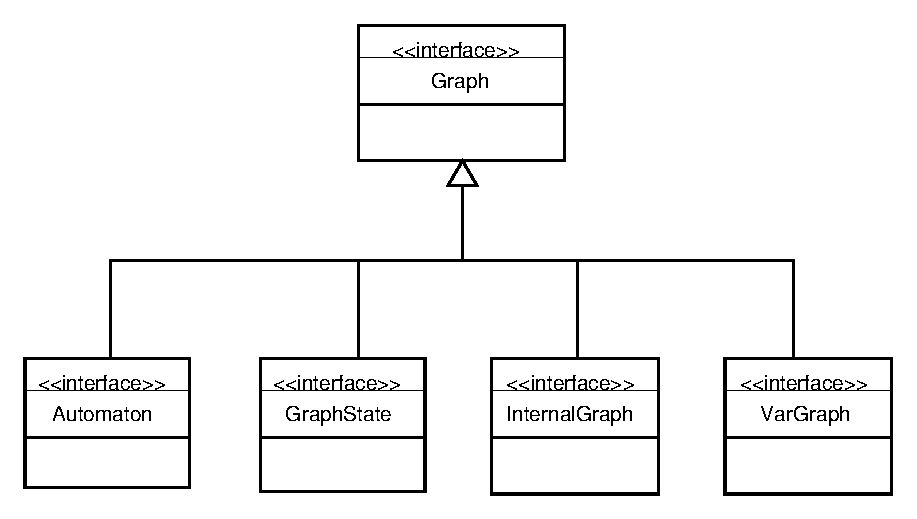
\includegraphics[scale=0.7]{\figdir/graph-hierarchy}
  \caption{The \Graph interface with different sub-interfaces.}
  \flabel{graph-hierarchy}
\end{figure}

Within the GROOVE Tool Set different implementations of graph structures are available. They mainly differ in the way they access their components. \fref{graph-hierarchy} gives an overview of the most frequently used graph implementations. For each of these we will explain the idea behind those specific implementations.

\subsection{Applied Patterns}

\subsubsection{Model View Controller}